
\begin{figure}[H]
  \centering
  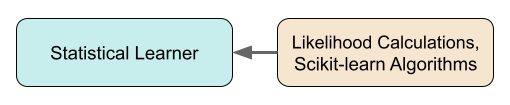
\includegraphics[width=0.7\linewidth]{./chapters/method/methodology3.png}
  \caption{Third portion of the flowchart from Figure \ref{fig:method} being 
           described in this section.}
\end{figure}

Choosing which algorithms to test is largely intuitive, but since this work has
yet to be benchmarked with simple algorithms, two straighforward algorithms
from the scikit-learn package \cite{scikit} were chosen and were introduced in
Section \ref{sec:algs}. Also covered in that section is the mathematical
framework of the \gls{MLL} calculation method. The implementation details of
these three approaches are covered here. 

\subsection{Scikit Algorithms}
\label{sec:scikit}

For many, the default behavior was retained. Prior to training, the data set is
preprocessed by scaling and normalization because the nuclide concentrations
vary by many orders of magnitude. Algorithm implementations from a python-based
\gls{ML} toolkit, scikit-learn \cite{scikit}, are used to train the models.

\subsection{Maximum Log-Likelihood Calculations}
\label{sec:mll}

\gls{MLL} Implementation
